\documentclass[12pt]{article}


\usepackage[dvips,letterpaper,margin=0.75in,bottom=0.75in]{geometry}
\usepackage{cite}
\usepackage{slashed}
\usepackage{graphicx}
\usepackage{amsmath}

\usepackage[american,fulldiode]{circuitikz}
\usetikzlibrary{calc}

\begin{document}
\ctikzset{bipoles/thickness=1}
\ctikzset{bipoles/length=.6cm}

\title{Transistor Parameters and Curves}

\maketitle

\begin{figure}[htbp]
\begin{center}
\begin{circuitikz}[american,line width=1pt]
\draw
(0,0) node[npn](npn1){} 
(npn1.C) to[R,l_=$R_C$,v^>=$V_2$,-*] ++(0,+1.5) coordinate(A) to[short,-o] ++(0,0.5) node[right]{$V_{\rm CC}$}
(npn1.C) to[short,*-o] ++(0.5,0) node[right]{$V_C$}
(npn1.E) to[short,-*] ++(0,-1.5) coordinate(B) node[ground,yscale=2.0]{}
(npn1.B) to[short] ++(-0.75,0) coordinate(C) to[R,l=$R_B$,v>=$V_1$] ++(-2.0,0) coordinate(D) 
(npn1.B) to[short,*-o] ++(0,0.5) node[above]{$V_B$}
(D) to[short,*-] ++(0,0.75) to[R,l_=$R_1$] ++(0,1.0) |- (A)
(D) to[short] ++(0,-0.75) to[R,l=$R_2$] ++(0,-1.0) |- (B)
;
\end{circuitikz} 
\caption{A transistor characterization circuit.}
\label{fig:beta}
\end{center}
\end{figure}


\begin{figure}[htbp]
\begin{center}
\begin{tabular}{c@{\hskip 0.5cm}c}
\begin{circuitikz}[american,line width=1pt]
\draw
(0,0) node[npn](npn1){} 
(npn1.C) to[R,l_=$R_C$,v^>=$V_2$,-*] ++(0,+1.5) coordinate(A) to[short,-o] ++(0,0.5) node[right]{$V_{\rm CC}$}
(npn1.C) to[short,*-o] ++(0.5,0) node[right]{$V_C$}
(npn1.E) to[short,-*] ++(0,-1.5) coordinate(B) node[ground,yscale=2.0]{}
(npn1.B) to[short] ++(-0.75,0) coordinate(C) to[R,l=$R_B$,v>=$V_1$] ++(-2.0,0) coordinate(D) 
(npn1.B) to[short,*-o] ++(0,0.5) node[above]{$V_B$}
(D) to[short,*-] ++(0,0.75) to[R,l_=$R_1$] ++(0,1.0) |- (A)
(D) to[short] ++(0,-0.75) to[R,l=$R_2$] ++(0,-1.0) |- (B)
(C) to[C,l=C,*-] ++(0,-1.0) to[sinusoidal voltage source,bipoles/length=1.25cm,l=$v_{\rm in}$,-*] ++(0,-1.25)
;
\end{circuitikz} &
\begin{circuitikz}[american,line width=1pt]
\draw
(0,0) node[ground,yscale=2.0]{} to[sinusoidal voltage source,bipoles/length=1.25cm,l=$v_{\rm in}$] 
++(0,2.0) to[C,l=$C$] ++(1.5,0)
to[R,l=$R_\pi$,v<=$v_{\rm be}$] ++(0,-2.0)
to[short,-*] ++(6.0,0) node[ground,yscale=2.0]{}
to[R,l=$R_C$] ++(0,2.0) coordinate(X) to[short,*-o] ++(0.5,0) node[right]{$v_{\rm out}$}
(X) to[short] ++(-1.25,0) coordinate(X) to[R,l_=$R_O$,*-*] ++(0,-2.0)
(X) to[short] ++(-1.5,0) coordinate(X) to[I,l_=$g_m v_{\rm be}$,bipoles/length=1.25cm,-*] ++ (0,-2.0)
;
\end{circuitikz} \\
(a) & (b) \\
\end{tabular}
\caption{A transistor characterization circuit (a) as built, and (b) in the hybrid-pi small signal approximation.}
\label{fig:char}
\end{center}
\end{figure}


\section{Pre-lab Calculations}
\noindent
1) For the circuit in Fig.~\ref{fig:char}, show that:
\begin{displaymath}
\beta = \left( \frac{R_B}{R_C} \right) \cdot \frac{V_2^Q}{V_1^Q}
\end{displaymath}
and derive an ``engineering formula'' for quickly calculating $\beta$ form the measured values of 
$V_2^Q$ and $V_1^Q$. \\

\noindent
2) Using the hybrid-pi small signal model for the circuit in Fig.~\ref{fig:char} show that the small signal gain in the limit that $C \to \infty$ and $R_0 \to \infty$ is given by:
\begin{displaymath}
\frac{|v_{\rm out}|}{|v_{\rm in}|} = g_m R_C
\end{displaymath}
and further that:
\begin{displaymath}
g_m R_C = \frac{V_2^Q}{nV_T} 
\end{displaymath}
and so we should expect to observe:
\begin{displaymath}
\frac{|v_{\rm out|}}{|v_{\rm in}|} = \frac{V_2^Q}{nV_T}
\end{displaymath}\\

\noindent
3) Calculate the corner frequency for the voltage divider formed by $C$ and $R_\pi$ at the input of the transistor in Fig.~\ref{fig:char}b.


\begin{figure}[htbp]
\begin{center}
\begin{tabular}{c@{\hskip 2cm}c}
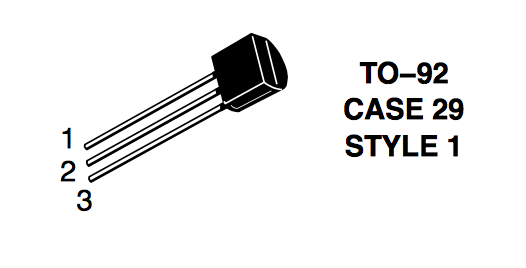
\includegraphics[height=0.10\textheight]{figs/case3904.png} &
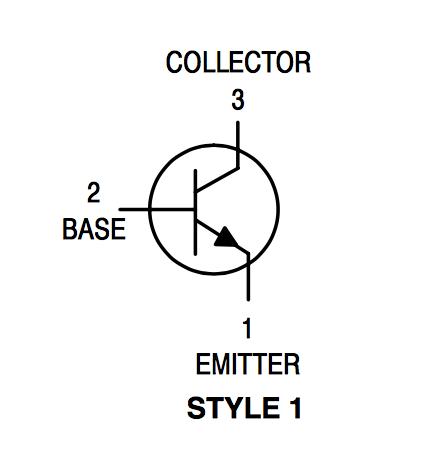
\includegraphics[height=0.18\textheight]{figs/pinout3904.png} \\
\end{tabular}
\end{center}
\caption{The TO-92 Style 1 package used for some discrete transistors,
including the 2N3904 (NPN) and 2N3906 (PNP) transistors used throughout this lab.  Note that
not all transistors use the same pinout, even if they are in the TO-92
package.}
\label{fig:layout}
\end{figure}

\section{Introduction}

In this lab, you will quantitatively evaluate the transistor current gain ($\beta$) model and the hybrid-pi model for the transistor.  You will also build a transistor current mirror,  which works based on the principle of transconductance.

\section{Current Gain Model}

Build the circuit in Fig.~\ref{fig:beta} using a 2N3904 NPN transistor, $R_1=220~\rm \Omega$ $R_2=R_C=100~\Omega$, and $R_B = 10~\rm k\Omega$.  Set the DC voltage $V_{\rm CC}$ provided by your bench-top DC power supply to $5~\rm V$.  Check the voltage drop across the Base-Emitter junction, and ensure that it is approximately a diode drop (0.7~\rm V).

Measure $V_1$ and $V_2$ using your DMM.  Use the engineering formula derived in pre-lab to calculate the $\beta$ parameter for this transistor.  Repeat this measurement for two more transistors, and record all of your answers.  If case you aren't seeing variation larger than $20\%$, the instructor has put aside a few outliers for you to measure.

Keep your favorite transistor and return the others to the draw, but take note of the $\beta$ of the transistor which you have kept for further study.

\section{Transconductance Model}

Now build the circuit in Fig.~\ref{fig:char}a from your existing circuit by connecting your function generator to the transistor base via a capacitor with $C=0.1~\rm \mu F$.  We are going to use this circuit to make a series of measurements demonstrating the linear relationship between the transconductance $g_m$ and the quiescent collector current $I_C^Q$.

Using alligator clips, attach your DMM  to monitor the DC voltage across the resistor $R_C$, from which you can determine $I_C^Q$.  Setup your oscilloscope with both ground probe shields connected to ground, the channel one probe tip at $V_{\rm B}$, and the channel two probe tip at $V_{\rm C}$.  Set both channels to AC coupling, so that you are monitoring the small AC signals $v_B$ and $v_C$.  In the transconductance model, the AC gain between these two points is given by $\frac{v_C}{v_B} = g_m R_C$ if we assume that $R_0$ is very large.

Setup your function generator to produce a $10~\rm kHz$ sine wave with an RMS voltage of $10~\rm mV$.  Now adjust the voltage of your supply (staying below $5~\rm V$) to make a series of measurements at the quiescent points $V_2^Q=400~\rm mV, 300~\rm mV, 200~\rm mV, 100~\rm mV$.  At each point, record the DC voltage $V_2^Q$ and the RMS AC voltages (as measured on your scope) for $v_C$ and $v_B$.  

At each point, compute the observed gain for the transistor $v_C/v_B$ and compare to the expected value for gain $g_m R_C = v_2^Q / (n V_T)$ where we can take $n=1$ and $V_T=26~\rm mV$.

By what factor do these estimates differ?  What value of the ideality factor would account for this?  The reported value for the ideality factor for this transistor is nearly one (1.01).  What else could account for this discrepancy?

\section{Transresistance}

Leave your scope to measure the quiescent bias current, but move your scopes to monitor $v_{\rm in}$ (before the capacitor) and $v_{\rm B}$ (after the capacitor).  Now adjust the voltage of your supply (staying below $5~\rm V$) to make two measurements at the quiescent points $V_2^Q=400~\rm mV, 100~\rm mV$.  At each quiescent point, record the DC voltage $V_2^Q$ and adjust the frequency of the function generator until you find the corner frequency where $v_{\rm B} = 0.7 v_{\rm in}$.  Record this frequency.

Calculate the input impedance $R_{\rm \pi}$ using the formula you calculated in pre-lab and compare to the theoretical value of our model 
\begin{displaymath}
R_{\rm \pi} = \beta/g_m = \beta \frac{n V_T} { I_C^Q}.
\end{displaymath}

\section{Transistor Current Source}

\begin{figure}[htbp]
\begin{center}
\begin{tabular}{c@{\hskip 0.25in}c}
\begin{circuitikz}[line width=1pt]
\draw
(0,0) node[pnp](pnp1){} 
++(-2,0) node[pnp,xscale=-1.0](pnp2){}
(pnp2.E) to[short,-*] (pnp1.E) to [short,-o] ++(0,0.5) node[right]{$V_+$}
(pnp1.B) to[short] ($(pnp1.B)!0.5!(pnp2.B)$) coordinate(A) to[short,*-] (pnp2.B)
(A) |- (pnp1.C) to[R,l=$R_{\rm P}$,*-] ++(0,-1.5) node[ground,yscale=2.0]{} 
(pnp2.C) node[left]{$P_{\rm src}$} to[R,l=$R_{\rm L}$,o-] ++(0,-1.5) node[ground,yscale=2.0]{} 
;
\end{circuitikz} &
\begin{circuitikz}[line width=1pt]
\draw
(0,0) node[left]{$V_+$} to[I,l=$I_{\rm src}$,bipoles/length=1.25cm,o-o] ++ (0,-2)
node[right]{$P_{\rm src}$} to[R,l=$R_{\rm L}$,o-] ++(0,-1.5) node[ground,yscale=2.0]{} 
%++(-2,0) node[pnp,xscale=-1.0](pnp2){}
%(pnp2.E) to[short,-*] (pnp1.E) to [short,-o] ++(0,0.5) node[right]{$V_+$}
%(pnp1.B) to[short] ($(pnp1.B)!0.5!(pnp2.B)$) coordinate(A) to[short,*-] (pnp2.B)
%(A) |- (pnp1.C) to[R,l=$R_{\rm P}$,*-] ++(0,-1.5) node[ground,yscale=2.0]{} 
%(pnp2.C) node[left]{$P_0$} to[R,l=$R_{\rm L}$,o-] ++(0,-1.5) node[ground,yscale=2.0]{} 
;
\end{circuitikz} \\
(a) & (b) \\
\end{tabular}
\caption{Current mirror circuit.}
\label{fig:current}
\end{center}
\end{figure}

Build the circuit in Fig.~\ref{fig:current} using two 2N3906 PNP transistors and $R_P = 220~\rm k\Omega$.

Test your circuit using using $R_L = R_P$ and $R_L = R_P/10$.  You should observe that the voltage at $P_{\rm src}$ changes by about an order of magnitude when you change the load by this amount.  Therefore, the circuit behaves more like a current source than a voltage source.

\section{Lab Report}

Your report should include all of your measurements and a comparison with your calculation.
 
\end{document}
